%=================
\chapter{Sprint 2}
%=================

%-------------------
\section{Pre-sprint}
%-------------------
Sprint 1 gave the desired result, but the team was not satisfied with the way the Scrum process was conducted, especially the sprint planning. In sprint 1 retrospect we decided to conform more to, in our mind, proper Scrum. Applying experience and advice from the first sprint, to get a better process. 

This planning meeting we will try to have more descriptive work items in the sprint backlog. This will ease the process of design, implementation, testing and documentation of the utility, and we do not have to redo any parts that will end up in the report in order to assist the reader. We focus on good user stories to ensure that the elements are low enough level.


%------------------------
\section{Sprint Planning}
%------------------------
The first sprint resulted in a solid core for the utility. During the next sprint iteration, the core will be extended with more advanced functionality. After this sprint, the utility will have most of the functionalities it need to work in a real environment, and will probably be able to aid Thales in some of their operations.

Not yet understanding the complexity of all the requirements in the sprint backlog, the team ended in an uncertain person-hours estimate for some work objects. Time will show if we understood the complexity and assigned enough hours to implement it. The more complex, but not so critical functionalities will be part of sprint 3 and 4.   

\subsection{Duration}
%--------------------
According to the work breakdown structure, \autoref{tab:wbs}, the planning meeting of the second sprint should have been conducted the 5th of October. After a request from the customer to see our planning for the second sprint at the weekly customer meeting, which was scheduled to be before our planning meeting the same day, we decided to advance the planning to the 4th of October. This is to maintain the good relationship to the customer and submit to their preference.

The sprint started with the planning meeting the 4th of October and our work started the following day. The sprint duration is 14 days, and will end the 18th of October with a review meeting.  

\subsection{Sprint Goal}
%-----------------------
The second sprint will build on the core created in the first sprint. During the sprint we will extend the functionality with more comprehensive and advanced features. Most of the requirements we intend to fulfill in this sprint had to be done subsequent to the first sprint, because the structure and design of the core had to be in place first. The requirements that are selected for this sprint is a natural advancement on the way to make the utility that the customer wants. 

One of the most crucial functions to work in a real environment, is the support for nested header-files. The handling of the \#include-statement gives the utility this feature. The goal of the sprint is to implement the \#include and mainly to have support for enums, bit streams, endianness and batch mode. 

\subsection{Back Log}
%--------------------
\label{sec:sp2backlog}
The second sprint we will implement thirteen requirements. These are listed in Table
\ref{tab:sprint2req1} and Table \ref{tab:sprint2req2}.

\begin{table}[!htb] \small \center
\caption{Sprint 2 Requirements\label{tab:sprint2req1}}
\begin{tabularx}{\textwidth}{l l X c c}
	\toprule
	& & & \multicolumn{2}{c}{Hours} \\
	\cmidrule(r){4-5}
	\# & Req. & Description & Est. & Act. \\
	\midrule
	1 & FR1-B & Support members of type enums & \underline{ 6 } & 5 \\
	   &  & Implementation & 3 & 2 \\
	   &  & Testing - unit & 1 & 1 \\
	   &  & Testing - end to end & 2 & 2 \\
	\addlinespace
	2 & FR1-C & Support members of type structs & \underline{ 7 } & 3.5 \\
	   &  & Implementation & 6 & 3 \\
	   &  & Testing - unit & 1 & 0.5 \\
	\addlinespace
	3 & FR1-F & Detect structs with same name & \underline{ 3 } & 3.5 \\
	   &  & Implementation & 2 & 2.5 \\
	   &  & Testing - unit & 1 & 1 \\
	\addlinespace
	4 & FR2-B & Support display of structs within structs & \underline{ 11 } & 15 \\
	   &  & Implementation & 5 & 6 \\
	   &  & Testing - unit & 2 & 2 \\
	   &  & Testing - end to end & 4 & 7 \\
	\addlinespace
	5 & FR4-F & Support enumerated named values & \underline{ 5 } & 6.5 \\
	   &  & Design & 1 & 0.5 \\
	   &  & Implementation & 1 & 0.5 \\
	   &  & Testing - unit & 1 & 2.5 \\
	   &  & Testing - end to end & 1 & 1.5 \\
	   &  & User documentation & 1 & 1.5 \\
	\addlinespace
	6 & FR4-G & Support for bit strings & \underline{ 10 } & 11.5 \\
	   &  & Design & 2 & 2 \\
	   &  & Implementation & 3 & 6 \\
	   &  & Testing - unit & 2 & 1 \\
	   &  & Testing - end to end & 2 & 1 \\
	   &  & User documentation & 1 & 1.5 \\
	\addlinespace
	7 & FR1-E & Support members of type array & \underline{ 7 } & 12 \\
	   &  & Implementation & 3 & 7 \\
	   &  & Testing - unit & 1 & 1 \\
	   &  & Testing - end to end & 3 & 4 \\
	\bottomrule
\end{tabularx}
\end{table}

\begin{table}[!htb] \small \center
\caption{Sprint 2 Requirements continued\label{tab:sprint2req2}}
\begin{tabularx}{\textwidth}{l l X c c}
	\toprule
	& & & \multicolumn{2}{c}{Hours} \\
	\cmidrule(r){4-5}
	\# & Req. & Description & Est. & Act. \\
	\midrule
	8 & FR4-E & Structs with various trailers & \underline{ 18 } & 15 \\
	   &  & Design & 3 & 2 \\
	   &  & Implementation & 6 & 6 \\
	   &  & Testing - unit & 2 & 1.5 \\
	   &  & Testing - end to end & 5 & 3.5 \\
	   &  & User documentation & 2 & 2 \\
	\addlinespace
	9 & FR4-B & Support for custom Lua configuration & \underline{ 14 } & 7 \\
	   &  & Design & 2 & 1 \\
	   &  & Implementation & 5 & 5 \\
	   &  & Testing - unit & 1 & 0 \\
	   &  & Testing - end to end & 4 & 1 \\
	   &  & User documentation & 2 & 0 \\
	\addlinespace
	10 & FR4-D & Dissector ID & \underline{ 4 } & 3 \\
	   &  & Implementation & 1 & 1 \\
	   &  & Testing - unit & 1 & 1 \\
	   &  & User documentation & 2 & 1 \\
	\addlinespace
	11 & FR5-C & Endian handling & \underline{ 11 } & 0.5 \\
	   &  & Implementation & 5 & 0.5 \\
	   &  & Testing - unit & 2 & 0 \\
	   &  & Testing - end to end & 6 & 0 \\
	\addlinespace
	12 & FR6-C & Batch processing; folder support in the CLI & \underline{ 7 } & 4.5 \\
	   &  & Implementation & 4 & 2 \\
	   &  & Testing - unit & 2 & 1.5 \\
	   &  & User documentation & 1 & 1 \\
	\addlinespace
	13 & FR4-C & Support custom handeling of specific data types & \underline{ 5 } & 3 \\
	   &  & Implementation & 2 & 1.5 \\
	   &  & Testing - unit & 1 & 0.5 \\
	   &  & Testing - end to end & 1 & 1 \\
	   &  & User documentation & 1 & 0 \\
	\addlinespace
	14 &  & Non-requirement programming tasks & \underline{ 26 } & 25.5 \\
	   &  & Refactoring & 3 & 7 \\
	   &  & Bug fixing & & 2 \\
	   &  & Manual end-to-end tests & 8 & 4 \\
	   &  & Automatic end-to-end tests & 4 & 3 \\
	   &  & Misc unit tests & 4 & 3 \\
	   &  & Misc user documentation & 7 & 6.5 \\
	\midrule
	& & Total: & 134 & 115.5 \\
	\bottomrule
\end{tabularx}
\end{table}


\begin{table}[!htb] \small \center
\caption{Sprint 2 Timetable\label{tab:sprint2time}}
\begin{tabularx}{\textwidth}{X c c}
	\toprule
	& \multicolumn{2}{c}{Hours} \\
	\cmidrule(r){2-3}
	Description & Est. & Act. \\
	\midrule
	\textbf{Sprint planning} & \textbf{30} & \textbf{35.5} \\
	\addlinespace
	\textbf{Sprint 2 requirements} & \textbf{134} & \textbf{115.5} \\
	Design & 8 & 5.5 \\
	Implementation & 44 & 43 \\
	Testing & 46 & 35 \\
	User Documentation & 10 & 6.5 \\
	Other & 26 & 25.5 \\
	\addlinespace
	\textbf{Sprint review} & \textbf{20} & \textbf{17.5} \\
	\addlinespace
	\textbf{Report documentation} & \textbf{58} & \textbf{69} \\
	Sprint 1 document & 14 & 5 \\
	Sprint 2 document & 44 & 54 \\
	Report document & & 10 \\
	\addlinespace
	\textbf{Lectures} & \textbf{25} & \textbf{27.5} \\
	\addlinespace
	\textbf{Meetings} & \textbf{55} & \textbf{48} \\
	Advisor meetings & 28 & 26 \\
	Customer meetings & 6 & 8 \\
	Stand-up meetings & 21 & 14 \\
	\addlinespace
	\textbf{Project Managment} & \textbf{20} & \textbf{40} \\
	\midrule
	Total: & 342 & 353 \\
	\bottomrule
\end{tabularx}
\end{table}




%----------------------
\section{System Design}
%----------------------
For sprint 2 the team decided to refactor some of the code in order to make it easier to read and to split the functionalities of the utility in such a way that it reduces coupling within the system.Some new functionality was also added on the parser side in order to get the utility to recognize the datatypes mentioned in the sprint 2 backlog. This new functionality is represented in the by the addition of new classes in the dissector and config modules. These classes include the BitField, ArrayField,EnumField and ProtocolField classes, which contain the functionality required to handle Bitstrings, arrays, enums and structs within structs respectively. The classes added to the config module include the Trailer, Bitstring, Custom and Enum classes which handles the configuration needs for structs with trailers, bitstrings, custom handling of data types and enums respectively. Other than that, there were no other changes or additions made to the design during sprint 2.

\subsection{Utility}
%--------------------
\autoref{fig:sp2:class} shows the class diagram the team made for sprint 2. The main differences from sprint 1 are the additions of new classes, extending the functionality of the utility so that the utility can handle more complex header files than it could before. The developers also generalized some of the modules and used inheritance to support the re-use of code 
\begin{figure}[!htb]
	\center
	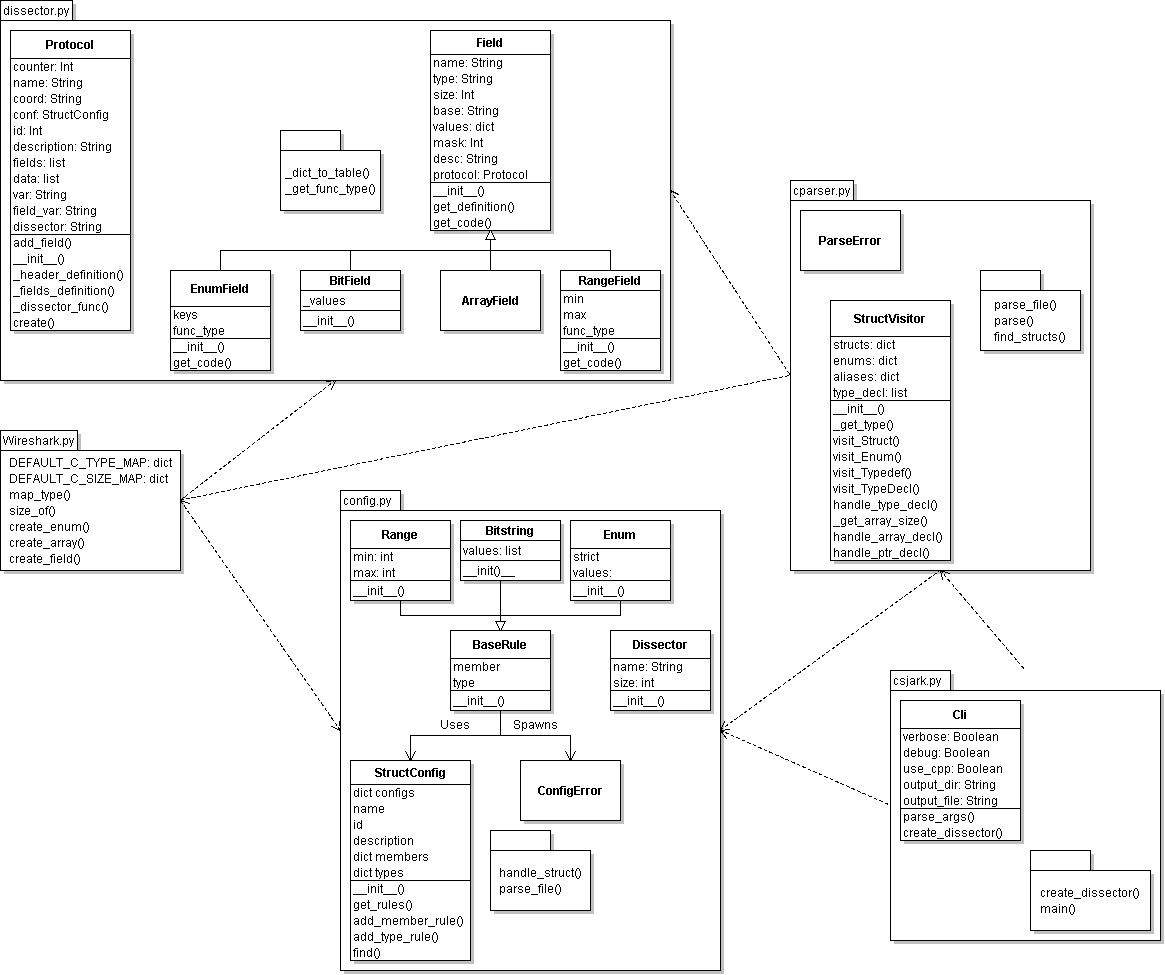
\includegraphics[width=\textwidth]{./sprints/img/class_diagram_s2}
	\caption{Class Diagram\label{fig:sp2:class}}
\end{figure}

%----------------------
\section{Implementation}
%----------------------

In the previous sprint we focused on creating a naive implementation of the 
utility. In this sprint the focus was on implementing data types for the 
C programming language and making it possible to configure more options on how 
the dissector will function. This section will cover the requirements 
implemented, how they were implemented and what the ''output'' looks like.

\subsection{Support Members of Type enum}
%----------------------
\label{sec:supportenum}
Enum is a type declaration in C, which specifies enumeration constants.  Enum 
is supported because it is a basic datatype in the C language. 
\autoref{code:cenum} shows an example of an enum in a C-header file. The 
Wireshark dissector will display the named value, making it 
easier to read, an example is shown in \autoref{fig:wscenum}. The red 
rectangle shows the enumerated named value.

\begin{figure}[ht]
	\center
	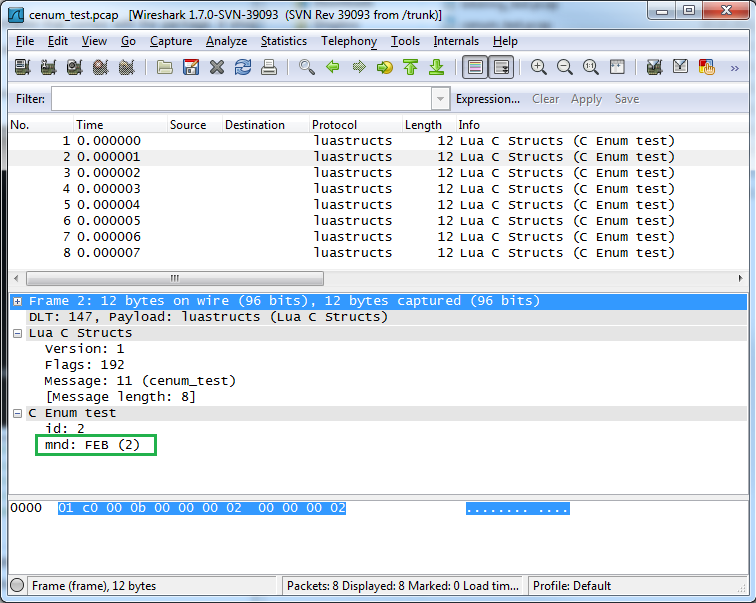
\includegraphics[width=\textwidth]{./sprints/img/wireshark_cenum}
	\caption{Enumeration in Wireshark\label{fig:wscenum}}
\end{figure}

\lstset{language=C,caption={Enum support},label=code:cenum}
\lstinputlisting[language=C]{./sprints/code/cenum_test.h}

\subsection{Support Members of Type Struct}
%----------------------
Structs are an important part of the C language, a struct declaration consists 
of a group of different fields, these fields can have any type, also struct. 
This was therefore an important requirement to implement. An example is shown 
in \autoref{code:structmember}.

\lstset{language=C,caption={Struct support},label=code:structmember}
\lstinputlisting[language=C]{./sprints/code/struct_member.h}

\subsection{Detect Structs with Same Name}
%----------------------
Two structs can have the same name, and therefore we needed a way of detecting it. 
If the parser finds two structs with the same name, an exception is 
raised, and the generation of the dissector is terminated.

\subsection{Support display of structs within structs}
%----------------------
The utility is able to display structs within a struct in Wireshark, the 
member will be visible, and the struct will be in a subtree that can be 
expanded. \autoref{fig:wsstructstruct} is a screenshot of this dissector in 
Wireshark.

\begin{figure}[ht]
	\center
	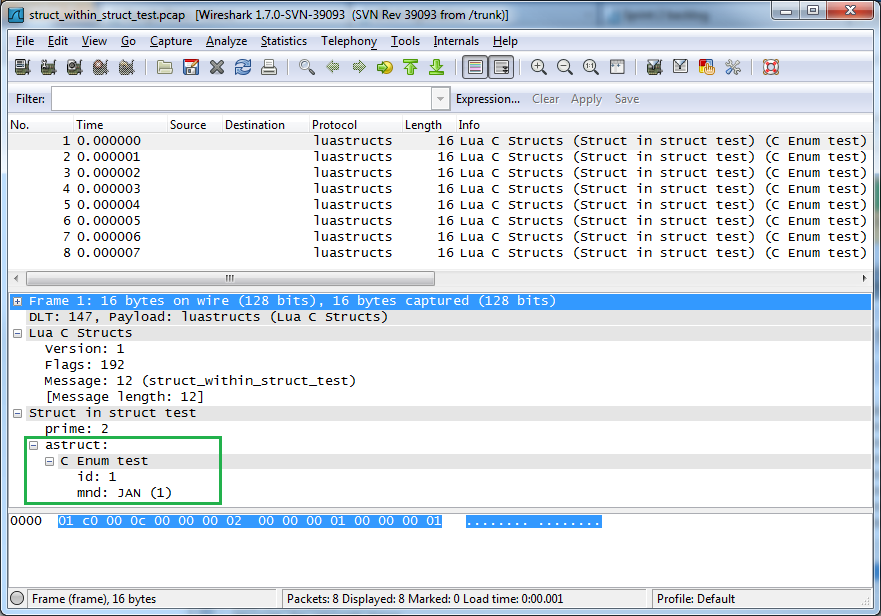
\includegraphics[width=\textwidth]{./sprints/img/wireshark_structwithstruct}
	\caption{Structs in Wireshark\label{fig:wsstructstruct}}
\end{figure}

\subsection{Support Enumerated Named Values}
%----------------------
In C there are two ways to do enumerations, the first option was explained in 
\autoref{sec:supportenum}, the other way is to use \#define which is shown in 
\autoref{code:defenum}. The advantage of using \#define is that the values 
can be generated. Since this cannot be understood by the parser, it can be 
generated directly from the header file, so it have to be supported by 
configuration. \autoref{code:enumconf}. The Lua-dissector will display the 
enum in the same way as in \autoref{sec:supportenum}.

\lstset{language=C,caption={Enumerated named values},label=code:defenum}
\lstinputlisting[language=C]{./sprints/code/def_enum.h}

\lstset{language=C,caption={Enumerated named values config},label=code:enumconf}
\lstinputlisting[language=C]{./sprints/code/def_enum.yml}

\subsection{Support for Bit Strings}
%----------------------
All bits in a basic data type can represent different values. An integer is 
represented by 4 bytes(32 bits), each of these bits can for example represent 
32 ''true/false' values. Our utility support configuration of these bits. Bits 
can be in groups, so they can represent more than two values. 
\autoref{code:bitstring} shows how bit string can be configured. 
\autoref{fig:wsbitstring} shows an example of how bit strings are displayed in 
Wireshark. Each group of bits are masked, so it is easier to see the values. 
The values are also named, if they are configured.

\begin{figure}[ht]
	\center
	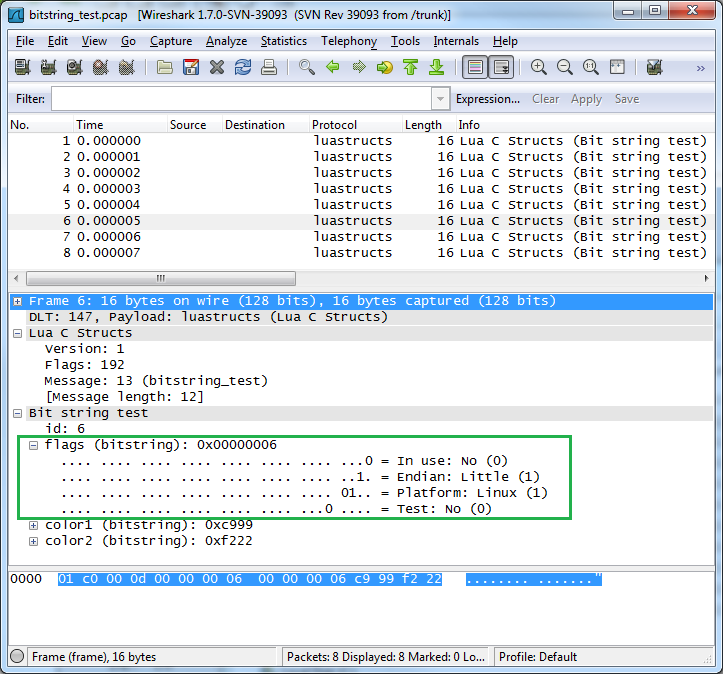
\includegraphics[width=\textwidth]{./sprints/img/wireshark_bitstring}
	\caption{Bit string in Wireshark\label{fig:wsbitstring}}
\end{figure}

\lstset{language=C,caption={Bitstring configuration},label=code:bitstring}
\lstinputlisting[language=C]{./sprints/code/bitstring.yml}

\subsection{Support Members of Type Array}
%----------------------
Csjark supports header-files with arrays, and is able to display them in 
Wireshark with the Lua-dissector. Csjark supports arrays of all data types 
implemented so far. The Wireshark dissector can display multidimensional 
arrays, and will create a new subtree for each dimension.  A representation of 
arrays in wireshark is displayed in \autoref{fig:wsarray}.

\begin{figure}[ht]
	\center
	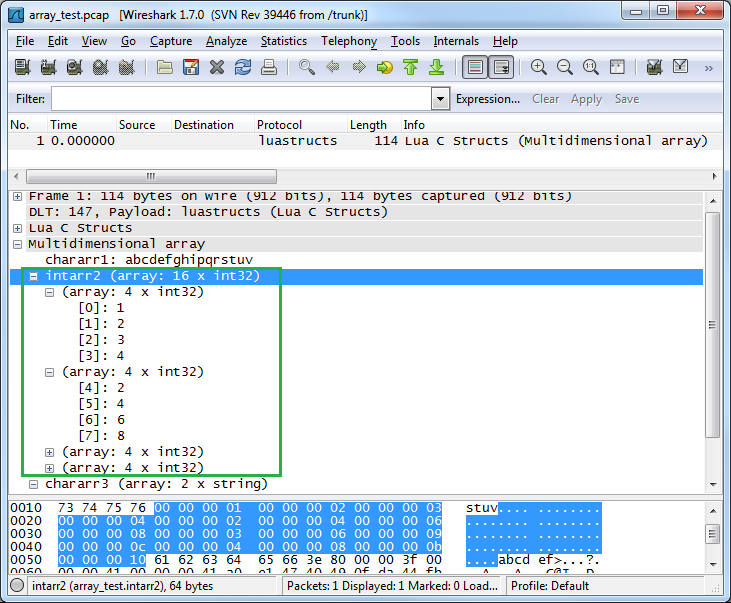
\includegraphics[width=\textwidth]{./sprints/img/wireshark_array}
	\caption{Arrays in Wireshark\label{fig:wsarray}}
\end{figure}

\subsection{Struct with Various Trailers}
%----------------------
The utility is able to support all kinds of trailers, that wireshark has 
built-in dissector for. Trailers are data that follows a struct, this can be 
any kind of data, but only trails that have built-in support in wireshark can 
be displayed.  To be able to use the wireshark dissectors, they have to be 
configured. In the example below, the wireshark dissector for ASN.1 
BER\footnote{Basic Encoding Rules}  is used.  In \autoref{code:trailer}, we 
specify ''asn1\_count'' as a member in the struct, this is used to tell the 
number of ASN.1 fields. The config in  \autoref{code:trailerconf} specifies 
fields with size of six bytest, the number of fields are specified by the data 
sent with the struct. At the end there is aa field of size five bytes. An 
example of ASN.1 in wireshark, can be seen in \autoref{fig:wstrailer}.

\begin{figure}[ht]
	\center
	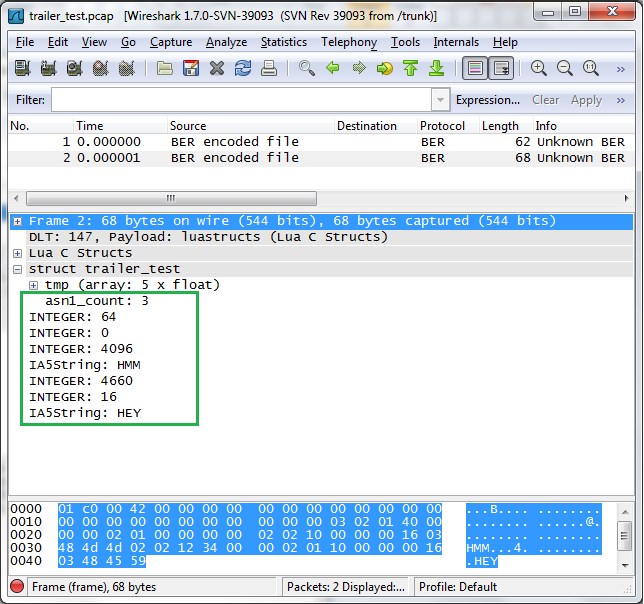
\includegraphics[width=\textwidth]{./sprints/img/wireshark_trailer}
	\caption{BER Trailer in Wireshark\label{fig:wstrailer}}
\end{figure}

\lstset{language=C,caption={Enumerated named values},label=code:trailer}
\lstinputlisting[language=C]{./sprints/code/trailer.h}

\lstset{language=C,caption={Enumerated named values config},label=code:trailerconf}
\lstinputlisting[language=C]{./sprints/code/trailer.yml}

\subsection{Custom Lua Configuration}
%----------------------
Csjark can support custom Lua configuration, by including Lua-scripts from a 
file specified in the configuration file. The reason for supporting custom Lua 
configuration is for protocols that are not built-in dissectors in Wireshark, 
and are not structs. The only way to support this, is to write a own dissector 
in Lua, and include it in the configuration. 
TODO: Not finished(add example + screenshot)

\subsection{Dissector ID}
%----------------------
All struct-packets that Wireshark captures, has a header, one of the fields in 
the header is the message id. This id is used to load the the correct 
dissector when a packet is captured. Each dissector should have a unique id, 
to avoid possible conflicts. This functionallity is implemented and the 
message id must be specified in the configuration file, \autoref{code:msgid} 
is an example of how this is done.

\lstset{language=C,caption={Dissector ID config},label=code:msgid}
\lstinputlisting[language=C]{./sprints/code/messageid.yml}

\subsection{Endian Handling}
%----------------------
Endian handling is postponed to the next sprint, because it is a platform 
specific problem, and should be implemented together with platform support.

\subsection{Folder Support in the CLI}
%----------------------
Folder support in the CLI\footnote{Command-line Interface} has been 
implemented, so it is possible to generate Lua-scripts for all structs stored 
in a given folder. At the moment, all dissectors will be regenerated. 
Functionality to only generate modified or new header-files will be added in 
the next sprint. \autoref{fig:csjarkfolder} is an example usage of CSjark where
the command first shows the usage of CSjark, and the second command 
generates dissectors from the folder ''header/'' and configurations from ''etc/''.

\begin{figure}[ht]
	\center
	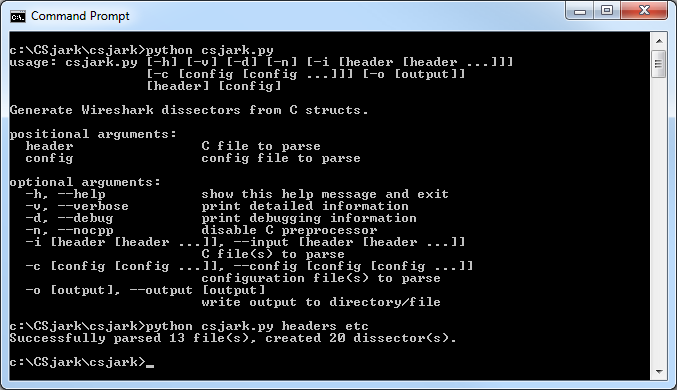
\includegraphics[width=\textwidth]{./sprints/img/csjark_folder}
	\caption{Arrays in Wireshark\label{fig:csjarkfolder}}
\end{figure}

\subsection{Support Custom Handling of Specified Data Types}
%----------------------
The utility supports custom handling of specific data types, this includes 
functionality to support  time\_t and nstime\_t. All basic data types and 
struct members can be configured to be handled in a special way. 
\autoref{code:customstruct} show an example of a struct with four members, two 
of them are time fields, and the last two is a BOOL and an integer to be 
handled in a custom way. This struct is configured in 
\autoref{code:customconfig}, in the config the two time fields are configured 
to be respectively absolute time and relative time, and the BOOL type to have 
a size of four bytes. The struct member ''all' is configured with an enumerated 
value, and will be visible as a hex-value. \autoref{fig:customdatatype} is a 
screenshot of the struct in Wireshark.

\begin{figure}[ht]
	\center
	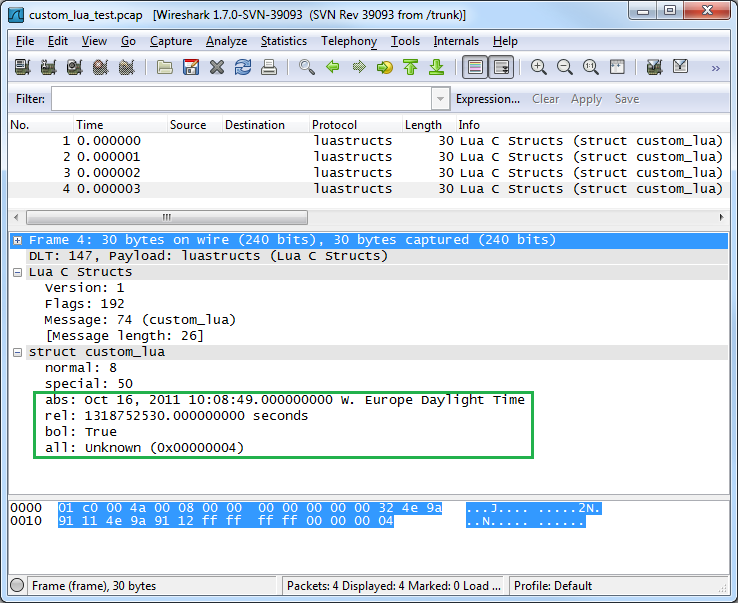
\includegraphics[width=\textwidth]{./sprints/img/wireshark_custom}
	\caption{Custom handling of Data Typesk\label{fig:customdatatype}}
\end{figure}

\lstset{language=C,caption={Struct for custom handling},label=code:customstruct}
\lstinputlisting[language=C]{./sprints/code/customfield.h}

\lstset{language=C,caption={Config for custom handling},label=code:customconfig}
\lstinputlisting[language=C]{./sprints/code/customfield.yml}

\subsection{Typedef Support}
%----------------------
Csjark is supporting the keyword typedef, which is a facility to create new 
data types names. \autoref{code:typedef} shows examples of typedef's that 
csjark supports.

\lstset{language=C,caption={Typedef example},label=code:typedef}
\lstinputlisting[language=C]{./sprints/code/typedef.h}

%-----------------------
\section{Sprint Testing}
%-----------------------
This section introduces the tests preformed during the sprint and their results. For sprint 2 it was also decided that the larger unit tests should also be documented and added to the test documents.

%subsection{Tests}
During the sprint the team executed a total of 6 tests with names as seen below. Tests executed:
\begin{itemize}
	\item TID08 - Supporting members of type enum \autoref{tab:sp2TID08}
	\item TID09 - Supporting members of type array  \autoref{tab:sp2TID09}
	\item TID10 - Supporting the display of structs within structs  \autoref{tab:sp2TID10}
	\item TID11 - Supporting enumerated named values  \autoref{tab:sp2TID11}
	\item TID12 - Supporting bit strings  \autoref{tab:sp2TID12}
	\item TID13 - Supporting structs with various trailers \autoref{tab:sp2TID13}
	\item TID14 - Sprint 2 functionality test \autoref{tab:sp2TID14}
\end{itemize}

\subsection{Test Results}
%----------------------------
\begin{table}[!htb] \footnotesize \center
\caption{Recognizing Supporting enums \label{tab:sp2TID08}}
\begin{tabular}{l l}
	\toprule
	Header & Description \\
	\midrule
	Description &  Supporting members of type enum  \\
	Tester & Lars Solvoll Tønder \\
	Date & 15.10.2011 \\
	Result & Success\\
	\bottomrule
\end{tabular}
\end{table}

\begin{table}[!htb] \footnotesize \center
\caption{Recognizing Supporting arrays \label{tab:sp2TID09}}
\begin{tabular}{l l}
	\toprule
	Header & Description \\
	\midrule
	Description &  Supporting members of type array   \\
	Tester & Lars Solvoll Tønder \\
	Date & 15.10.2011 \\
	Result & Success\\
	\bottomrule
\end{tabular}
\end{table}

\begin{table}[!htb] \footnotesize \center
\caption{Supporting the display of sctructs within structs \label{tab:sp2TID10}}
\begin{tabular}{l l}
	\toprule
	Header & Description \\
	\midrule
	Description &  Supporting the display of sctructs within structs \\
	Tester & Erik Bergersen \\
	Date & 17.10.2011 \\
	Result & Success. \\
	\bottomrule
\end{tabular}
\end{table}

\begin{table}[!htb] \footnotesize \center
\caption{Supporting enumerated name values \label{tab:sp2TID11}}
\begin{tabular}{l l}
	\toprule
	Header & Description \\
	\midrule
	Description &  Supporting enumerated name values \\
	Tester & Lars Solvoll Tønder \\
	Date & 17.10.2011 \\
	Result & Success\\
	\bottomrule
\end{tabular}
\end{table}


\begin{table}[!htb] \footnotesize \center
\caption{ Supporting bit strings \label{tab:sp2TID12}}
\begin{tabular}{l l}
	\toprule
	Header & Description \\
	\midrule
	Description & Supporting bit strings \\
	Tester & Lars Solvoll Tønder \\
	Date & 17.10.2011 \\
	Result & Success\\
	\bottomrule
\end{tabular}
\end{table}

\begin{table}[!htb] \footnotesize \center
\caption{Supporting structs with various trailers \label{tab:sp2TID13}}
\begin{tabular}{l l}
	\toprule
	Header & Description \\
	\midrule
	Description & Supporting structs with various trailers \\
	Tester & Erik Bergersen \\
	Date & 18.10.2011 \\
	Result & Success\\
	\bottomrule
\end{tabular}
\end{table}

\begin{table}[!htb] \footnotesize \center
\caption{Sprint 2 functionality test\label{tab:sp2TID14}}
\begin{tabular}{l l}
	\toprule
	Header & Description \\
	\midrule
	Description & unit test covering all of the functionality implemented in sprint 2 \\
	Tester & Lars Solvoll Tønder \\
	Date & 18.10.2011 \\
	Result & Success\\
	\bottomrule
\end{tabular}
\end{table}

\subsection{Test Evaluation}
%-------------------------------
For the second sprint the developers focused a lot more on testing during implementation. The team also decided that the testers should check how much of the code was covered in the unit tests. This made the group focus more on making proper unit tests that tests as much functionality as possible This had a very positive effect on the tests ran at the end of the sprint where not a single test failed, except for one test which ended up exposing a bug in Wireshark

\subsubsection{Test Coverage}
This section introduces the amount of code covered by our unit tests and how it relates to the test coverage from the previous sprints.
 MAKE A GRAPH OF THE CODE COVERAGE AND PUT IT HERE

 


%--------------------------
\section{Customer Feedback}
%--------------------------
\subsection{Requirement changes and feedback}
In sprint 2 we were able to demonstrate many of the requirements for the customer, and as a result we got some feedback of some changes and refinements that the customer wants. The customer also added some new features they would like to have. The changes and additions are listed bellow.

\subsubsection{FR1-E: Support members of type array}
Arrays should be displayed as a sublevel. Multidimensional arrays should have one sublevel per dimension. The dissector should also display the type of the array and show the different indexes for the sublevels.

\subsubsection{FR2-B: struct within structs}
The customer stated that the inner struct should be displayed as a sublevel of the outer struct.
When an external dissector is called, it should be called with name, and not id, so that structs that is never used as a base does not need to be assigned an id.

\subsubsection{FR4-C Custom handling of specific types}
The customer stated that they would like certain types to be interpreted in a certain way as default behaviour, but that the user should be able to configure specific behaviour for a specific member of a struct.

\subsubsection{FR4-E: Headers/trailers}
The customer originally stated that this feature included both headers and trailer structs for a given struct. This is now refined to mean that the given struct is the header, and that it can have various trailers (could be one or more c structs, ASN.1, etc.). A configuration file should specify the kind of trailer, and what variable inside the header struct which specify how many trailer items to expect. If the header does not specify the length of the trailer the dissector should just use the rest of the buffer, or the dissector is responsible to return the length used from the buffer, so the caller can give the rest to the next dissector.
In Wireshark it should be displayed as a sequence of structs.

\subsubsection{FR4-F: Support for integers that represents enumerated values and bit strings}
The customer clarified this by explaining that they wanted integers that represents an enumerated value to be displayed like an enum (member name and the string that represents the integer value) and that the bit strings should be displayed as a list with the name and value (1 / 0 or yes / no) of the different bits in the integer. It should also display the original integer I hex. As a result of this, the requirement was split into two:
\begin{itemize}
\item FR4-F	Support enumerated named values
\item FR4-G	Support for bit strings
\end{itemize}
The customer also confirmed that the bit strings are endian specific and that he would like then to start counting from 1 (not zero, as in our first implementation).

\subsubsection{FR5-C Endian handling}
The customer stated that the header part of the packed, which include the platform flag, will always be in big endian (network order).

\subsubsection{FR7-C: Batch mode}
The customer clarified this to mean that the utility should be able to run completely unattended given a set of command line arguments. For example it should not ask the users any questions under this modus. This is to be able to run it as a cron job at night.

\subsubsection{NR4: A user without prior knowledge should be able to use the tool within X hours.}
The customer defined X as 5.

\subsubsection{NR5: A user with prior knowledge should be able to use the tool within Y hours.}
The customer defined Y as 1.

\subsubsection{Detecting ambiguous struct definitions (more than one struct definition with the same name)}
The utility should detect if there are more that one struct with the same name. If found, the utility should exit with a proper error message because 

\subsubsection{Data alignment}
The customer said that we could have some problems with alignment with the current offsets, because the different platforms may pad the data members of a struct to match an integer number of words on that platform.

\subsubsection{Testability}
The customer suggested that we might want to refine some of the requirement to make them more testable. This can be done by adding more measurable goals.

\subsubsection{Documentation}
The documentation should specify what parameters are needed, like what parameters that should be passed to a dissector.

\subsubsection{Locating “missing” header files}
Some of the header files specified in a file might be located in an unknown location. The customer suggested that we should include a way to configure header location.

\subsubsection{What headers should the utility be generate dissectors for}
The customer suggested that we include a way to specify the relevant header files in a configuration file.

\subsubsection{Dissector id}
Only structs explicitly configured with an id should be assigned an id. The rest should be called by their textual name. This is to avoid id collisions and limit configuration needed.

\subsubsection{Headers and configuration the utility cannot handle}
The customer stated that they wanted the tool to continue generating dissectors even if it encounters a file it cannot handle. The tool should just give an appropriate error message and carry on with the next file.

\subsection{Customers feedback on the product}
The customer is satisfied with the progress of the utility and is so far pleased with its functionality. They also feel that the team are flexible when it comes to feature refinement and additions. 

%--------------------------
\section{Sprint Evaluation}
%--------------------------
This section contains the team evaluation of the second sprint.

\subsection{Review}
%--------------------------
The first sprint evaluation resulted in some planned actions for the forthcoming sprints. Looking back at these at now, we quickly realized that we fell into the same pitfalls again: lack of documentation, bad work distribution and reverse engineering of vital parts.

The sprint started out very good. We had a four-hour long planning meeting, and ended up with a good backlog and a common understanding of the technical aspects of the sprint. Even though the meeting was significantly better this time, we failed in doing the design early. User stories was postponed till the middle of the sprint and they were written by team members that had no understanding of the code. Doing them in a reverse engineered fashion ended up being more work than expected. This is something that we definitely have to change in the next sprints, if we want to do Scrum properly.

The rest of the sprint was as expected. Implementation went smoothly and the customer are satisfied of our progress.

The planned improvement in the documentation part was not followed up. We did more documentation than in the first sprint, but we had problems gathering it together so that the advisers could look at it. In this way we lost a lot of valuable feedback. We have to focus on this the next sprint.

In our sprint backlog, that we made at the sprint planning meeting, we listed responsible for each task. In retrospect this did not work out very well. The problem we encountered was that the most experienced programmer took almost all the programming tasks, leaving documentation tasks for the rest of the team. This could have worked out well, if the documentation and implementation were independent of each other. We know that the implementation and documentation are highly dependent, and that it is not easy to write documentation for code you have not written yourself. So all team members had to ask the implementer how he did it and how it works, which was not very efficient. 
This actually resulted in two bad experiences:
\begin{itemize}
\item Work distribution was uneven. Those with responsibilities were expected to do their task, but we did not think that a task might have been poorly estimated. Some tasks which seemed simple ended up being hard and consumed a lot of person hours.
\item Not all items in the sprint backlog were completed. Because of the uneven work distribution, we realised too late that some of the backlog items would take considerable more time to complete. The person responsible for a task might have had a lot of other tasks that he needed to complete before starting on the current task, and thereby he could not get help from the other team members to complete the it.
\end{itemize} 
 All in all we feel that we are still learning to do Scrum properly and if we take the new planned actions in true consideration, we most likely will perform considerable better at the next iteration. 
\\
\\
The burndown chart, \autoref{fig:sp2:burndown}, shows the progress during the second sprint. The estimation seem bad, but since we postponed one of the work items it does not reflect the true actual hours left. The postponed item was estimated 13 hours. Then the sprint end up being 27-13=14 actual hours left. We feel that the estimations, if we exclude the postponed work item, were good and accurate.
\begin{figure}[!htb]
	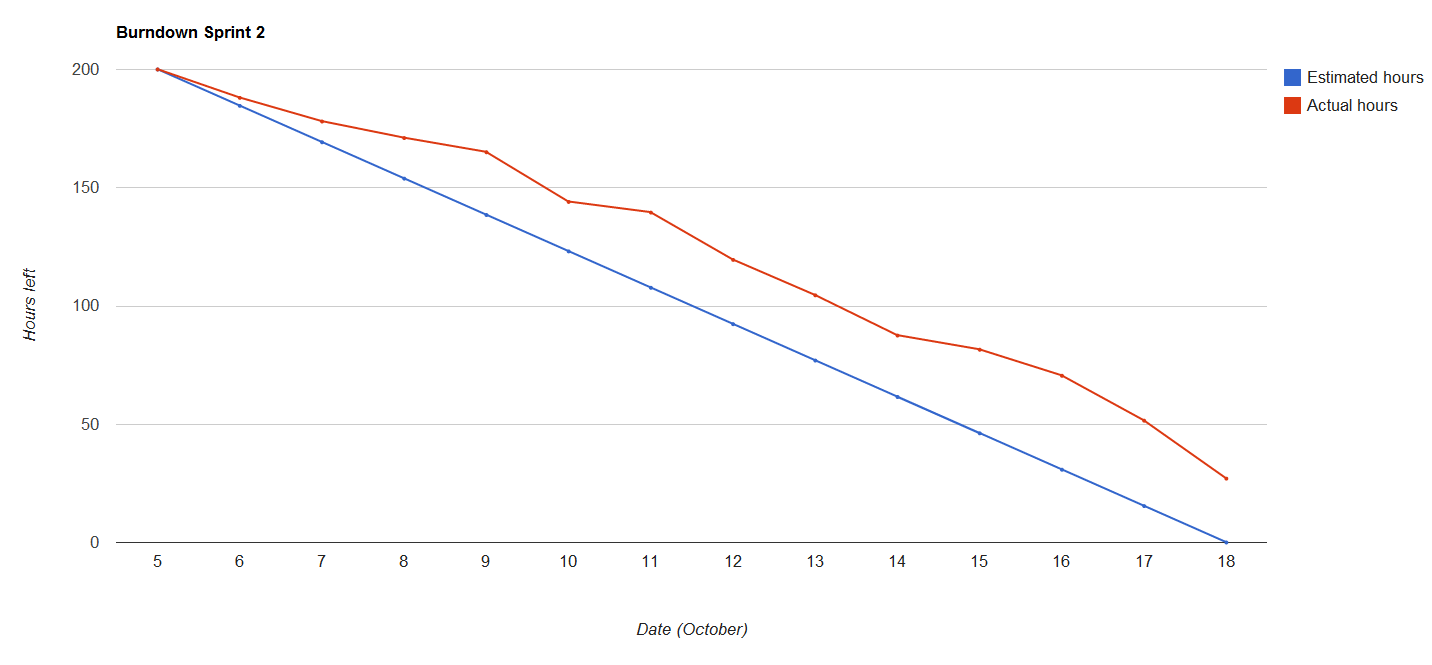
\includegraphics[width=\textwidth]{./sprints/img/burndown_chart_s2}
	\caption{Burndown chart\label{fig:sp2:burndown}}
\end{figure}



\subsection{Positive Experiences}
%--------------------------
\begin{itemize}
	\item A significantly better sprint planning meeting
	\item All the team members have raised their effort, working more hours
	\item Accurate time estimates for most of the work items
	\item Successful presentation of the utility to the customer
	\begin {itemize}
		\item Implementation of features are as intended
		\item Good feedback from the customer
	\end{itemize}
	\item Thriving team atmosphere
\end{itemize}



\subsection{Negative Experiences}
%--------------------------
\begin{itemize}
	\item The planning meeting was too short, which resulted in a shortcoming in the documentation.
	\item Documentation was postponed till the end again
	\item Lack of feedback to the advisor
	\item Bad work balance
	\item Could not complete all the tasks in the backlog
\end{itemize}


\subsection{Planned Actions}
%--------------------------
We intend to complete these planned actions for the next sprint. To achieve better performance it is crucial that the importance of these actions are not neglected.

\subsubsection{Do the design in the planning}
Last evaluation meeting we agreed to do the design early in the sprint. Since that did not work for us, we have decided to do the design IN the planning meeting. Then it will not be possible to postpone it and the rest of the work will be more efficient. We will use as many hours as it takes to have a planning meeting where we end up with a good plan, proper documentation and detailed user stories.

\subsubsection{Not assign responsibilities}
We will not assign responsibilities for all the tasks at the sprint planning meeting, we rather assign responsibilities for one task for each team member. This way no team members can assign themselves a lot of tasks and might in the end realize that they are not able to complete all the tasks. Now all team members will be able to see what is done and what is not, and assign an undone task to themselves. We hope that this will make us capable of completing the whole sprint backlog within the given time.

\subsubsection{List dependencies and prioritize the work items}
As some tasks are dependent on others, it is important to understand this early and plan so that no team member must wait for others to do a task. Now that we do not want to assign responsibilities to all tasks, it is crucial to prioritize each task so that we know what tasks to do first. We do not want to end up with undone work items that have a high priority when the sprint is over. These changes are applied to the sprint backlog.

\subsubsection{Provide more and better documentation to the advisers}
We will strive to give our advisers more documentation to look at. We need their feedback and help in order to finish this project in a suitable manner. 


\subsection{Barriers}
%--------------------------
\subsubsection{The work distribution} 
As mentioned in the review, the team had a uneven work distribution. Some team members were eager to start implementing and took all the implementation tasks, leaving mostly documentation tasks for the rest of the team. The documentation tasks are closely connected to the implementation, so this resulted in problems. Documentation were postponed till the end.The planned actions section describes how we are planning to avoid that this happens again. 

\subsubsection{Wireshark} 
We identified several bugs in Wireshark, which ended up crashing it when we tried to run our utility. Most of them were fixed by Stig, as he works as a core developer for Wireshark. Unfixed bugs either will be fixed or dropped because they are not really relevant to us. Time can be lost while we wait for a patch.

\subsubsection{Complexity consideration}
As always, design and estimation of future implementation is hard. At the planning meeting, we evaluated each work item and estimated the complexity of it. In hindsight we saw that our complexity consideration for some of the work items was wrong, making it hard to complete all the items in the sprint backlog.
